\chapter{Todo-rename-DNN}
\label{chap:dnn}
\section{Introduction}
The major Problem in \textit{Machine Learning} is that in most of real world applications, many factors of variation influence every single piece of data. Most of real world applications require us to disentangle these factors of variation in data and discard the ones which we don't care about. But it can be very difficult to extract these high level abstract features from raw data obtained. \textit{Deep learning} aims solves this problem in representation learning by introducing representations that are expressed in terms of other, simpler representations.

According to \cite{deng2014deep}, \textit{``Deep learning (deep structured learning or hierarchical learning) is a set of algorithms in machine learning that attempt to model high-level abstractions in data by using model architectures composed of multiple non-linear transformations"}.

Some of most successful deep learning methods uses principles \textit{Artificial Neural Networks (ANN)}. Different deep learning architectures which uses principles \textit{ANNs} such as Convolutional Neural Networks (CNNs), and Deep Belief Networks (DBN) have been applied to different  fields like computer vision, automatic speech recognition and  natural language processing where produced state-of-the-art results.

In this chapter we fist introduces Deep Neural Network and its bacic concepts in \ref{sec:dnn:dnn}. Later we briefly discuss common DNN architecture like \textit{CNNs, DBN, etc}.

\section{Deep Neural Network}
\label{sec:dnn:dnn}
Artificial neural networks are family of statistical learning models inspired by the \textit{1959 biological model (by Nobel laureates David H. Hubel \& Torsten Wiesel)}. A \textit{Deep Neural Network (DNN)} is a form of  Artificial Neural Network with multiple hidden layers between the input and output layers. 


\subsection{Motivations for Deep Architectures}
The Major motivations for deep architectures are the following:

\subsubsection{Deep architecture of Brain}
One of major motivation of Deep Architectures is deep structure of brain. For example, study of visual cortex, shows areas which contains representation of the input, and signals flow from one area to the next. Each level represents the input at a different level of abstraction, with more abstract features further up in the hierarchy, defined in terms of the lower-level ones. Moreover, representation in brain is between dense distributed and local: they are sparse (only 1\% of neurons are simultaneously active). 

\subsubsection{Insufficient depth can hurt}
According to complexity theory of circuit, deep architectures is more efficient than shallow architectures in terms of computational elements and parameters required to represent some functions. \citep{bengio2007scaling}. Haastad found that a function (of $n$ inputs) which can be efficiently represented with $O(n)$ nodes with a depth $d$, requires an exponential number ($O(2^n)$) of nodes if depth is $d-1$. \citep{bengio2007greedy}

\subsubsection{Cognitive processes seem deep}
If you consider process of perceiving by humans, we always organize ideas and concepts hierarchically.  we first learn simple concepts and then compose them to represent more abstract ones. 


\subsection{General Deep Network Framework}
As discussed in Section \ref{sec:dnn:dnn} Deep Neural Network can be considered as Multilayer perceptron with many hidden layers. Standard learning strategy of MLP contains following steps:
\begin{itemize}
\item The weights of Neural network is initialized by random values
\item Apply gradient descent using back-propagation (BP) algorithm.
\end{itemize}
But Apart from few exceptions, researchers soon found out that an MLP of more
than two hidden layers often failed \cite{bengio2007greedy} due to a well-known fact that the MLP learning involves an extremely difficult non-convex optimization problem and a gradient-based local search used in the BP algorithm easily gets stuck in local minimum.

So a greedy layer-wise training algorithm was proposed by \citet{hinton2006reducing} to train Deep Networks. It contain following major steps:
\begin{itemize}
\item Pre-training one layer at a time in a greedy way. This unsupervised learning at each layer in a way that preserves information from the input and disentangles factors of
variation in data. This act as initialization step. Hence, instead of doing a random initialization, we perform careful initialization and reduce chance of getting stuck on local minima.
\item Then network is fine-tuned with respect to the ultimate criterion of interest which may be classification or regression task.
\end{itemize}

\section{Deep Belief Networks}
Hinton showed that \emph{Restricted Boltzmann Machines (RBMs)} can be stacked and trained in a greedy manner to form so-called \emph{Deep Belief Networks (DBN)} \cite{hinton2006reducing}. Deep Belief Network is graphical model which learns to extract a deep hierarchical representation of data. First, an unsupervised training is performed on each layer (RBM) in a greedy manner. Then fine-tune network based on a supervised training criterion.
\begin{figure}[!ht]
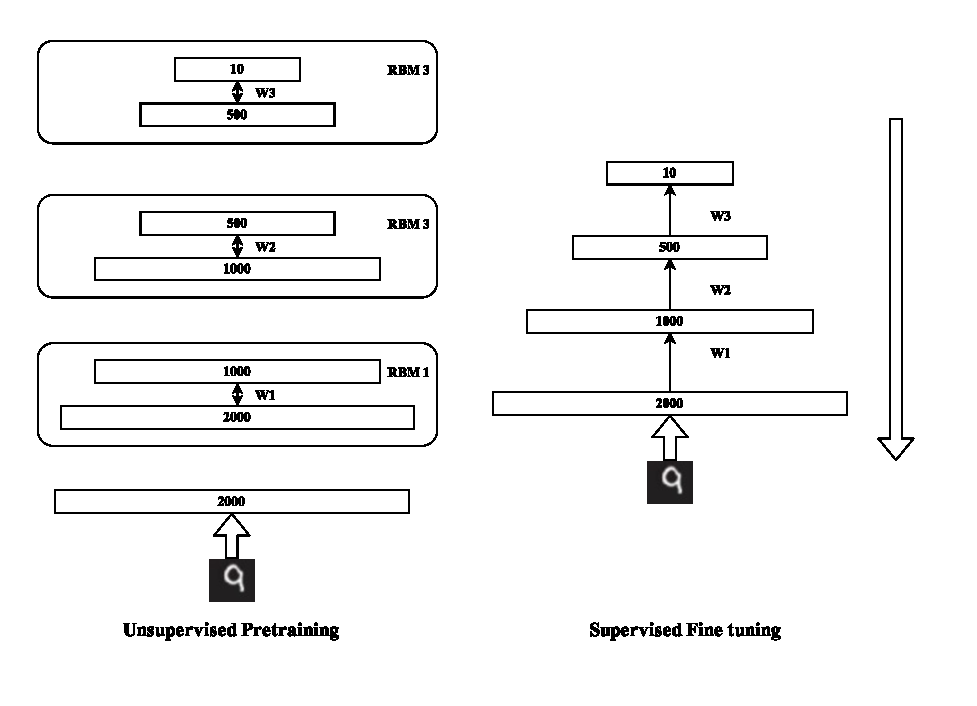
\includegraphics[scale=1]{./imgs/RBM_Train.eps} 
\caption{Training of DBN}
\end{figure}

RBM is an energy-based model. Energy based models has a scalar value (energy) to each configuration of variables. A graphical depiction of an RBM is shown in figure \ref{fig:rbm_layer}
\begin{figure}[!ht]
    \centering
    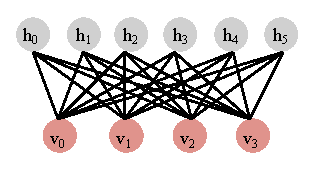
\includegraphics[scale=0.9]{./imgs/rbm.eps}
    \caption{A Restricted Boltzmann Machine Layer}
    \label{fig:rbm_layer}
\end{figure}%

The Energy function $E(v,h)$ is defined as 
$$E(v,h) = - b'v - c'h - h'Wv$$
where $W$ is weights between hidden and visible units and $b \& c$  are the offsets of the visible($v$) and hidden layers($h$) respectively. Like other Energy based model RBM also uses free energy (inspired from physics), which is defined as
$$\mathcal{F}(v) = -log \sum_{h}{e^{-(E(v,h))}}  $$
$$\mathcal{F}(v) = - b'v - \sum_i \log \sum_{h_i} e^{h_i (c_i + W_i v)}$$

Since hidden nodes and visible nodes are conditionally independent and binary units (where $v_j \& h_i \in \{0,1\}$), we have 
%\begin{equation} 
\begin{align}
p(h|v) &= \prod_i p(h_i|v) \\
p(v|h) &= \prod_j p(v_j|h) \\
P(h_i=1|v) &= sigm(c_i + W_i v) \label{eq:rbm_layers_prob1} \\
P(v_j=1|h) &= sigm(b_j + W'_j h) \label{eq:rbm_layers_prob2}  
\end{align}

And hence free energy is 
$$\mathcal{F}(v)= - b'v - \sum_i \log(1 + e^{(c_i + W_i v)})$$ %\label{eq:rbm_freeE}
Probability distributions over visible vectors are defined in terms of the free energy.
%p(v) = \frac {e^{-E(v)}} {Z} \text{ with } Z = \sum_v e^{-E(v)} \\
\begin{align*}
P(x) = \frac{e^{-\mathcal{F}(x)}}{Z} \text{ with } Z=\sum_x e^{-\mathcal{F}(x)}.
\end{align*}
Restricted Boltzmann machines are trained to maximize the product of probabilities assigned to some training set. It is usually difficult to determine this gradient analytically, as it involves the computation of $E_P[\frac{\partial \mathcal{F}(x)} {\partial \theta} ]$. This is nothing less than an expectation over all possible configurations of the input v (under the distribution P formed by the model). \cite{hinton2010practical}

A faster learning algorithm was proposed by Hinton \cite{hinton2002training,hinton2006reducing,hinton2010practical}. It starts by assigining the states of the visible units to a training vector. Then the states of hidden units are all computed in parallel using equation \ref{eq:rbm_layers_prob1}. Once binary states have been chosen for the hidden units, \textit{reconstruction} is produced by setting each $v_i$ to $1$ with a probability given by equation \ref{eq:rbm_layers_prob2}. This process is repeated for $k$ steps to produce $v'= v^{(k)}$ and $h' = h^{(k)}$. 

\begin{figure}[ht]
\centering
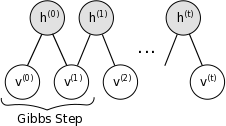
\includegraphics[width=0.3\textwidth]{./imgs/markov_chain.png}
\caption[Markov chain of training RBM layer]{Markov chain, that uses alternating Gibbs sampling for training RBM layer. As $t \rightarrow \infty$, samples $(v^{(t)}, h^{(t)})$ are guaranteed to be accurate samples of $p(v,h)$}
\label{fig:rbmmarkovChain}
\end{figure}

The change in the weights is given by
$$ \Delta W = \eta ({vh^\mathsf{T}}_{data} - {v'h'^{\mathsf{T}}}_{recon}). $$
where $\eta$ is learning rate. Outer product of $v$ and $h$ and called as the positive gradient and that of of $v'$ and $h'$ as negative gradient. A similar learning rule that uses the states of individual units is used for the adaption of biases. This process is called \textbf{Contrastive Divergence (CD-k)}. In practice, $k=1$ has been shown to work exceptionally well \cite{hinton2010practical}.

\section{Stacked Denoising Autoencoders}
\citet{vincent2010stacked} introduced the \emph{Stacked Denoising Auto-encoder (SdA)} which is an extension of the stacked auto-encoder. The denoising auto-encoders can be stacked to form a deep network by feeding the latent representation of the denoising auto-encoder found on the layer below, as input to the current layer. The unsupervised pre-training is done one layer at a time. Each layer is trained as a denoising auto-encoder by minimising the reconstruction error with respect of its input (which is the output code of the previous layer). Once all layers are \textit{pre-trained}, the network goes through a second stage of training called supervised \textit{fine-tuning} where we want to minimize prediction error on a supervised task.

The idea of auto-encoders has been part of the landscape of neural networks for decades. An auto-encoder is trained to encode the input $x$ into some representation $y = f(x)$ so that the input can be reconstructed from that representation. The auto-encoder has two components: the encoder $f:x \rightarrow y$ and the decoder $g:y\rightarrow z$. The reconstruction error can be computed in different ways, depending on the distributional assumptions on the input. More commonly used are:
\begin{itemize}
\item Traditional squared error.
$$ L(\mathbf{x} \mathbf{z}) = || \mathbf{x} - \mathbf{z} ||^2$$
\item If the inputs are either binary or considered to be binomial probabilities, then we can use cross-entropy of the reconstruction.
$$L(\mathbf{x}, \mathbf{z}) = - \sum^d_{k=1}[\mathbf{x}_k \log \mathbf{z}_k + (1 - \mathbf{x}_k)\log(1 - \mathbf{z}_k)]$$
\end{itemize}

The participle behind \emph{denoising autoencoders (dA)} is that, \textit{in order to force the hidden layer to discover more robust features and prevent it from simply learning the identity, we train the autoencoder to reconstruct the input from a corrupted version of it} \cite{vincent2008extracting}. The denoising auto-encoder can be viewed as a stochastic version of the auto-encoder. The stochastic corruption process randomly sets some of the inputs (probability is called corruption rate) to zero and tries to predict the original vector from the it's corrupted vectors. Hence, \textit{able to predict any subset of variables from the rest} is a sufficient condition for completely capturing the joint distribution between a set of variables.

\begin{figure}[ht]
\centering
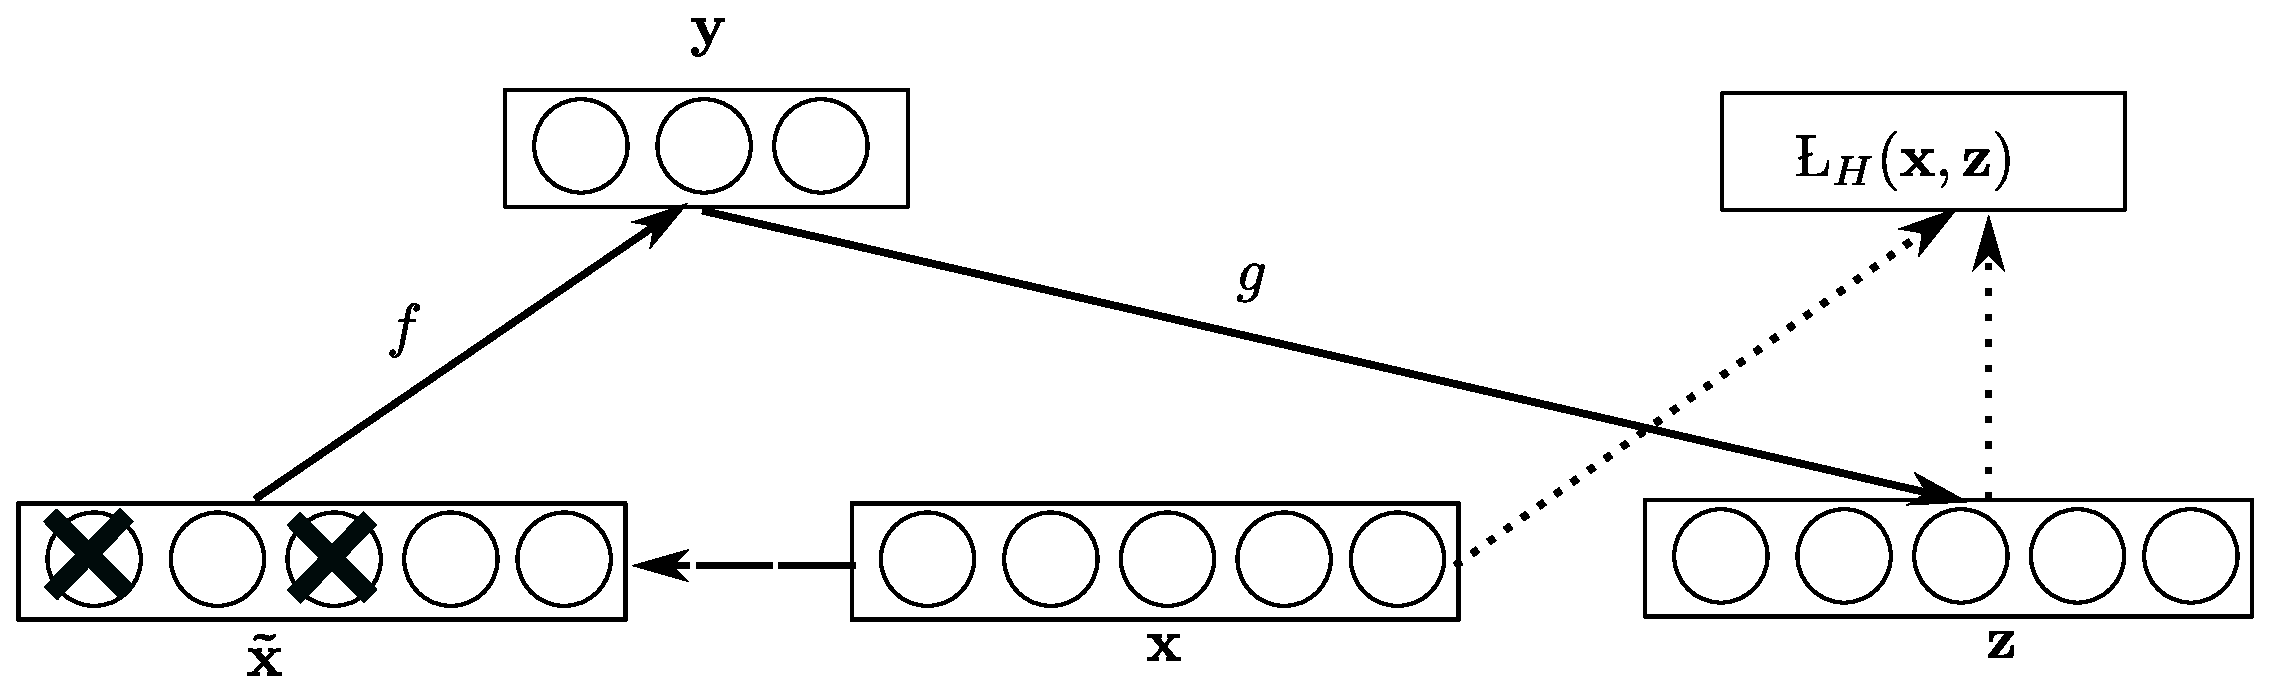
\includegraphics[width=0.8\textwidth]{./imgs/sda.eps}
\caption[The denoising autoencoder architecture]{The denoising autoencoder architecture. An example $\mathbf{x}$ is stochastically corrupted to $\mathbf{\tilde{x}}$. The autoencoder then maps it to $\mathbf{y}$ (via encoder $f$) and attempts to reconstruct $\mathbf{x}$ via decoder $g$, producing reconstruction $\mathbf{z}$. Reconstruction error is measured by loss $L_{H}(\mathbf{x},\mathbf{z})$. }
\label{fig:sdaChain}
\end{figure}

\section{Convolutional Neural Networks}
\emph{Convolutional Neural Network (CNN)} is a variant of Multilayer perceptron  and inspired by biological processes (From complex arrangement of cells in the cat’s visual cortex). Convolutional Neural Networks are designed to use less amount of preprocessing \cite{lecun1998gradient}. It was Introduced by Fukushima in 1980 and later  improved by \citet{lecun1998gradient}. CNNs are widely used as models for  image/video recognition. CNNs make use of local receptive fields, shared weights and spatial sub-sampling to ensure some degree of shift, scale and distortion invariant.

\noindent Two key idea of Convolutional Neural Network are
\begin{itemize}
\item \textsc{Sparse Connectivity:} The inputs of hidden units in layer $m$ are from a subset of units in layer $m-1$, units that have spatially contiguous receptive fields. This create a receptive field behavior and hence ensure that filters produce strong response to a spatially local pattern in input.


\item \textsc{Shared Weights:} Each filter $h_i$ of CNN is replicated. These replicated units share the same weight vector and bias and form a feature map. This not only reduces the number of free parameters to be estimated but also make CNN to learn position invariant feature detection.
\end{itemize}

\begin{figure}[!ht]
\centering
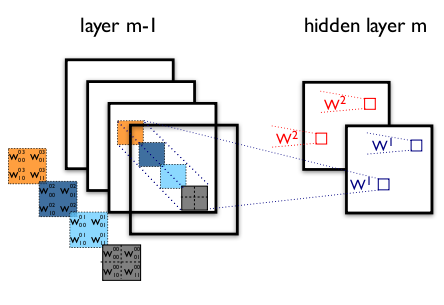
\includegraphics[width=0.6\textwidth]{./imgs/convolution.png} 
\caption[convolutional layer explained]{An example of a convolutional layer. Layer $m-1$ contains 4 feature maps and layer $m$ contains 2 feature maps ($h^0$ and $h^1$). Pixels in $h^0$ and $h^1$ (blue and red squares) are computed from pixels of layer $(m-1)$ which are within their $2\times2$ receptive field in the layer below (colored rectangles).}
\label{fig:cnn_layer}
\end{figure}


\noindent CNNs tries to capture high level feature of input images using following operations:
\begin{itemize}
\item \textsc{Convolution}: Most important operation of CNN is convolution. A \textit{feature map} is obtained by convolution of the input image with a linear filter and then applying a non-linear function. 
$$h^k_{ij} = fn( (W^k * x)_{ij} + b_k ).$$
Since this linear filter is applying repeatedly, the resulting connectivity act as a series of overlapping receptive fields
\item \textsc{Sub Sampling}: Sub-sampling refers to reducing the overall size of a signal. The most commonly used subsampling method is \textit{max pooling}. Max pooling divides the input into a set of non-overlapping sub-regions and, for each such sub-region, outputs the maximum value. It help in reduction of computation for higher layers. Moreover, it provides some form of translation invariance. 
\end{itemize}

\begin{figure}[!ht]
\centering
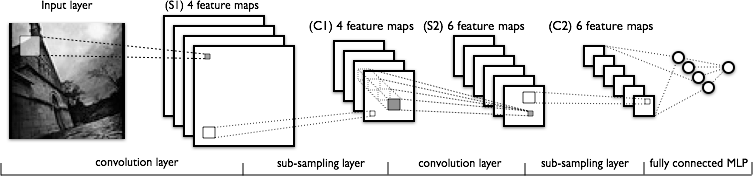
\includegraphics[width=0.9\textwidth]{./imgs/cnn1.png} 
\caption[An example of a convolutional neural network]{A typical example of a CNN \footnote{From site: http://white.stanford.edu/}. }
\label{fig:cnn_layer}
\end{figure}

Typically, Convolutional Neural Networks consists of a number of convolutional and subsampling layers optionally followed by fully connected layers (MLP). Some times we can use SVM instead of MLP. The input to a convolutional layer is a $m \times n \times r$ image where $m$ is the height and width of the image and $r$ is the number of channels (eg: 3 for RGB)/input feature maps. 
TODO: 3dCNN????????????
\section{Summary}
Deep learning algorithms attempts learn model high-level abstractions in data by help of multiple non-linear transformations. Deep Neural Networks is basically Artificial Neural Network with multiple hidden layers between input and output. Major characteristics  of Deep Learning are:
\begin{itemize}
\item They are usually Multilayered and Hierarchical.
\item They contains Multiple non-linear transformations 
\item They act as a feature extractors, they tries to high level abstract features from raw data.
\end{itemize}

Most of DNNs have greedy layer-wise training algorithm (pretraining) for initialization weights and followed by supervised fine-tuning.
 
Deep Belief Network is made of stacking of RBM layers. RBM attempts to reduce Free energy of network, and trained by Contrastive Divergence.
  
Denoising Auto-encodes can be stacked to form SdA. The aim of denoising Auto-encodes to predict the original data from the it's corrupted version.

Convolutional Neural Network contains a series of Convolution and sub sampling layers and optionally fully connected layer. CNN uses shared weights and spatial sub-sampling to ensure some degree of freedom from shift, scale and distortion of input.
